\documentclass[11pt,a4paper]{article}

% --- Essential Packages ---
\usepackage[utf8]{inputenc}
\usepackage[T1]{fontenc}
\usepackage{lmodern}
\usepackage[margin=0.85in, top=0.9in, bottom=0.9in]{geometry}
\usepackage{amsmath,amssymb}
\usepackage{xcolor}
\usepackage{graphicx}
\usepackage{booktabs}
\usepackage{tabularx}
\usepackage{array}
\usepackage{listings}
\usepackage{fancyhdr}
\usepackage{titlesec}
\usepackage{enumitem}
\usepackage{tcolorbox}
\usepackage{tikz}
\usetikzlibrary{shapes.geometric, arrows.meta, positioning, fit, backgrounds, calc}
\usepackage{hyperref}

% --- Geometry & Header Adjustments ---
\setlength{\headheight}{15pt}

% --- Color Palette ---
\definecolor{navyPrimary}{RGB}{15, 43, 72}
\definecolor{tealAccent}{RGB}{2, 132, 199}
\definecolor{darkSlate}{RGB}{51, 65, 85}
\definecolor{lightBg}{RGB}{248, 250, 252}
\definecolor{cardBorder}{RGB}{226, 232, 240}
\definecolor{alertAmber}{RGB}{217, 119, 6}
\definecolor{successGreen}{RGB}{5, 150, 105}
\definecolor{codeBg}{RGB}{241, 245, 249}
\definecolor{codeText}{RGB}{30, 41, 59}

% --- Typography & Section Styling ---
\titleformat{\section}
  {\color{navyPrimary}\normalfont\Large\bfseries}
  {\thesection}{1em}{}[\color{tealAccent}\titlerule]

\titleformat{\subsection}
  {\color{navyPrimary}\normalfont\large\bfseries}
  {\thesubsection}{1em}{}

\titleformat{\subsubsection}
  {\color{darkSlate}\normalfont\normalsize\bfseries}
  {\thesubsubsection}{1em}{}

% --- Header & Footer Configuration ---
\pagestyle{fancy}
\fancyhf{}
\fancyhead[L]{\textcolor{darkSlate}{\footnotesize \textbf{Drishti Platform} --- Non-Rooted Remote Access Architecture}}
\fancyhead[R]{\textcolor{darkSlate}{\footnotesize Technical Approach Specification}}
\fancyfoot[L]{\textcolor{darkSlate}{\footnotesize Confidential --- Internal Fleet Engineering}}
\fancyfoot[R]{\textcolor{darkSlate}{\footnotesize Page \thepage}}
\renewcommand{\headrulewidth}{0.4pt}
\renewcommand{\footrulewidth}{0.4pt}

% --- Hyperref Setup ---
\hypersetup{
    colorlinks=true,
    linkcolor=tealAccent,
    filecolor=tealAccent,
    urlcolor=tealAccent,
    citecolor=navyPrimary,
    pdftitle={Drishti: Non-Rooted Remote Device Access Architecture},
    pdfauthor={Drishti Fleet Systems Engineering},
    pdfsubject={Technical Approach Document for Unrooted Android Tablet Fleet Control}
}

% --- Custom Callout Boxes ---
\tcbuselibrary{skins,breakable}

\newtcolorbox{archbox}[1]{
    colback=lightBg,
    colframe=tealAccent,
    coltitle=white,
    fonttitle=\bfseries\small,
    title={#1},
    arc=2.5mm,
    boxrule=1pt,
    left=8pt,
    right=8pt,
    top=6pt,
    bottom=6pt,
    breakable
}

\newtcolorbox{alertbox}[1]{
    colback=lightBg,
    colframe=alertAmber,
    coltitle=white,
    fonttitle=\bfseries\small,
    title={#1},
    arc=2.5mm,
    boxrule=1pt,
    left=8pt,
    right=8pt,
    top=6pt,
    bottom=6pt,
    breakable
}

\newtcolorbox{successbox}[1]{
    colback=lightBg,
    colframe=successGreen,
    coltitle=white,
    fonttitle=\bfseries\small,
    title={#1},
    arc=2.5mm,
    boxrule=1pt,
    left=8pt,
    right=8pt,
    top=6pt,
    bottom=6pt,
    breakable
}

% --- Code Listings Configuration ---
\lstset{
    backgroundcolor=\color{codeBg},
    basicstyle=\ttfamily\footnotesize\color{codeText},
    breaklines=true,
    captionpos=b,
    commentstyle=\color{darkSlate}\itshape,
    keywordstyle=\color{tealAccent}\bfseries,
    stringstyle=\color{alertAmber},
    numbers=left,
    numberstyle=\tiny\color{darkSlate},
    numbersep=7pt,
    frame=single,
    rulecolor=\color{cardBorder},
    tabsize=2,
    showspaces=false,
    showstringspaces=false
}

% --- Document Metadata ---
\title{
    \vspace{-1.5cm}
    \begin{tcolorbox}[colback=navyPrimary,colframe=navyPrimary,arc=3mm,center,valign=center,top=10pt,bottom=10pt]
        \centering
        {\color{white}\Huge \textbf{DRISHTI REMOTE FLEET PLATFORM}}\\[6pt]
        {\color{tealAccent}\Large \textbf{Technical Approach Document: Zero-Root Android Fleet Operation}}\\[4pt]
        {\color{white}\small Architecture, Subsystem Pipelines, Device Owner Governance \& Installation SOP}
    \end{tcolorbox}
    \vspace{-0.5cm}
}
\author{\textbf{Drishti Systems \& Embedded Engineering Team}}
\date{\textbf{Document Revision:} 2.4 \quad | \quad \textbf{Target Platform:} Android 9.0 to 14+ (Unrooted Fleet)}

\begin{document}

\maketitle
\thispagestyle{fancy}

\begin{abstract}
\noindent Commercial interactive kiosks and vending machine deployments present a fundamental infrastructure dilemma: operators require reliable, 24/7 remote device management---including interactive screen sharing, unattended gesture injection, application lifecycle control, and diagnostic shell execution---yet hardware rooting poses prohibitive security, warranty, compliance, and stability liabilities. This document details the technical architecture and operational approach of the \textbf{Drishti Remote Access Platform} tailored specifically for \textbf{non-rooted Android tablet fleets}. 

By capitalizing on a single, deterministic, 10-second mounting-time USB provisioning step, the Drishti agent application is elevated to an \textbf{Android Enterprise Device Owner (DPM)}. This state fundamentally transforms the device's security model: dangerous permissions, MediaProjection background screen mirroring consent, and accessibility input dispatch are granted permanently and silently without human intervention. Screen streaming is executed via an adaptive, memory-efficient \textbf{MediaProjection/VirtualDisplay} pipeline, touch interactions are synthesized through a low-overhead \textbf{AccessibilityService} gesture injector, local debugging is enabled via an on-device embedded loopback ADB client, and all connectivity is routed through an \textbf{outbound-only reverse WebSocket tunnel} that reliably penetrates restrictive cellular firewalls and Carrier-Grade NAT (CGNAT). This approach eliminates the need for device rooting while achieving 100\% autonomous reboot persistence and enterprise-grade security.
\end{abstract}

\vspace{0.2cm}
\tableofcontents
\vspace{0.4cm}

% =============================================================================
\section{Executive Summary \& Problem Formulation}
% =============================================================================

\subsection{The Operational Context}
In distributed vending and automated retail networks, Android tablets function as primary customer-facing payment terminals, inventory displays, and telemetry controllers. Once mounted inside physical cabinetry, physical maintenance becomes exceptionally expensive, logistically complex, and disruptive to business operations. Technicians cannot be dispatched for routine software updates, diagnostic inspections, screen recalibrations, or application restarts.

Consequently, operators require three non-negotiable capabilities from an administrative web dashboard:
\begin{enumerate}[leftmargin=*]
    \item \textbf{Low-Latency Interactive Screen Sharing (VNC-Equivalent):} Real-time visual monitoring of tablet displays with sub-second feedback.
    \item \textbf{Unattended Remote Input Injection:} Full remote touch, swipe, keyboard, and system key dispatch directly from the web canvas into running third-party kiosk applications.
    \item \textbf{Remote Command \& Shell Diagnostics:} The ability to inspect logs, query hardware telemetry, install/uninstall APK packages, and restart services without physical device interaction.
\end{enumerate}

\subsection{The Rooting Dilemma in Enterprise Fleets}
Historically, remote support platforms achieved unattended device control by embedding a setuid root binary (\texttt{su}) or integrating custom OS ROMs. In a modern commercial vending fleet, rooting is fundamentally unacceptable for several critical reasons:
\begin{itemize}[leftmargin=*]
    \item \textbf{Security \& Compliance Vulnerabilities:} Vending tablets frequently interface with EMV payment peripherals, PCI-DSS payment gateways, and proprietary business logic. Rooting disables Android's SELinux enforcing mode, breaks application sandboxing, and exposes the hardware to privilege escalation exploits.
    \item \textbf{SafetyNet \& Play Integrity Failure:} Modern enterprise libraries, banking APIs, and protected media frameworks immediately refuse execution on rooted or compromised firmware.
    \item \textbf{OEM Warranty \& Support Invalidation:} Hardware vendors repudiate manufacturer warranties and remote RMA agreements if standard system partitions are unlocked or tampered with.
    \item \textbf{Firmware Brittleness Across OTA Updates:} Root patches frequently fail or cause catastrophic boot-loops when minor over-the-air (OTA) system updates are deployed by tablet manufacturers.
\end{itemize}

\begin{archbox}{Strategic Approach: The One-Time Physical Touch Advantage}
In vending machine operations, an engineer or field technician \textbf{must physically handle every tablet exactly once} during initial machine assembly and mounting. The Drishti platform exploits this guaranteed one-time physical access: by executing a single automated provisioning script over USB before final mechanical mounting, the agent APK is enrolled as the device's \textbf{Android Device Owner}. This one-time action permanently unlocks all necessary privileged capabilities on standard, factory-sealed, non-rooted hardware.
\end{archbox}

% =============================================================================
\section{High-Level Architectural Topology}
% =============================================================================

The Drishti platform is partitioned into three decoupled tiers: the on-device \textbf{Android Agent}, the scalable \textbf{Relay Backend}, and the administrative \textbf{Web Dashboard}. Figure~\ref{fig:arch} illustrates the operational topology.

\begin{figure}[htbp]
\centering
\resizebox{0.96\textwidth}{!}{%
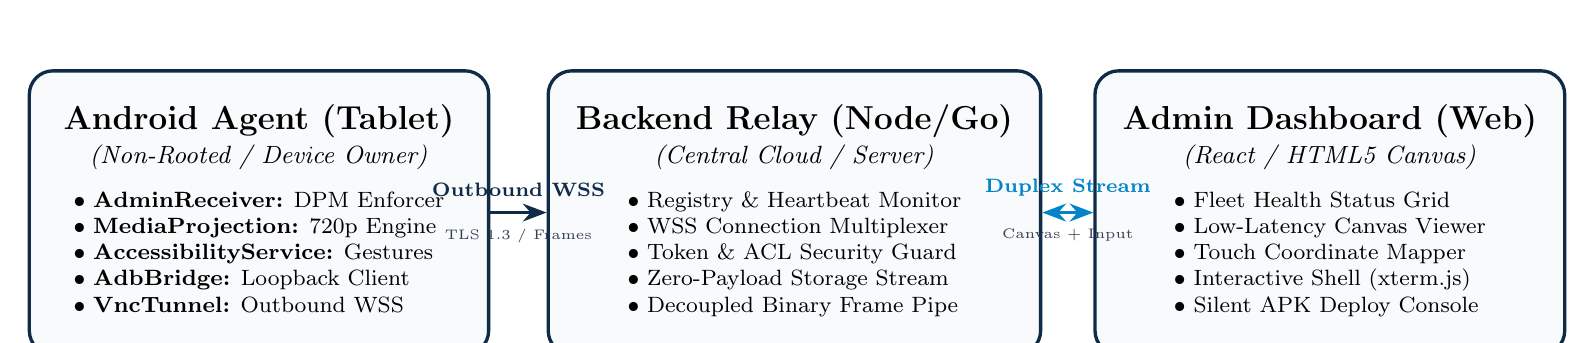
\begin{tikzpicture}[
    cloud/.style={draw=navyPrimary, rounded corners=3mm, fill=lightBg, line width=1.2pt, align=center, inner sep=10pt, minimum width=4.8cm, minimum height=3.6cm},
    arrow/.style={-{Stealth[length=3mm]}, line width=1.3pt, color=navyPrimary},
    biarrow/.style={{Stealth[length=3mm]}-{Stealth[length=3mm]}, line width=1.3pt, color=tealAccent}
]

% Nodes
\node[cloud, minimum width=4.5cm] (agent) at (0,0) {
    \textbf{\large Android Agent (Tablet)}\\
    \small \textit{(Non-Rooted / Device Owner)}\\[6pt]
    \footnotesize
    \begin{tabular}{l}
    $\bullet$ \textbf{AdminReceiver:} DPM Enforcer\\
    $\bullet$ \textbf{MediaProjection:} 720p Engine\\
    $\bullet$ \textbf{AccessibilityService:} Gestures\\
    $\bullet$ \textbf{AdbBridge:} Loopback Client\\
    $\bullet$ \textbf{VncTunnel:} Outbound WSS
    \end{tabular}
};

\node[cloud, minimum width=4.5cm] (backend) at (6.8,0) {
    \textbf{\large Backend Relay (Node/Go)}\\
    \small \textit{(Central Cloud / Server)}\\[6pt]
    \footnotesize
    \begin{tabular}{l}
    $\bullet$ Registry \& Heartbeat Monitor\\
    $\bullet$ WSS Connection Multiplexer\\
    $\bullet$ Token \& ACL Security Guard\\
    $\bullet$ Zero-Payload Storage Stream\\
    $\bullet$ Decoupled Binary Frame Pipe
    \end{tabular}
};

\node[cloud, minimum width=4.5cm] (frontend) at (13.6,0) {
    \textbf{\large Admin Dashboard (Web)}\\
    \small \textit{(React / HTML5 Canvas)}\\[6pt]
    \footnotesize
    \begin{tabular}{l}
    $\bullet$ Fleet Health Status Grid\\
    $\bullet$ Low-Latency Canvas Viewer\\
    $\bullet$ Touch Coordinate Mapper\\
    $\bullet$ Interactive Shell (xterm.js)\\
    $\bullet$ Silent APK Deploy Console
    \end{tabular}
};

% Connections
\draw[arrow] (agent.east) -- node[above=2pt, font=\scriptsize\bfseries, text=navyPrimary] {Outbound WSS} 
                           node[below=2pt, font=\tiny, text=darkSlate] {TLS 1.3 / Frames} (backend.west);

\draw[biarrow] (backend.east) -- node[above=2pt, font=\scriptsize\bfseries, text=tealAccent] {Duplex Stream} 
                                node[below=2pt, font=\tiny, text=darkSlate] {Canvas + Input} (frontend.west);

\end{tikzpicture}%
}
\caption{Drishti End-to-End System Topology for Non-Rooted Fleets.}
\label{fig:arch}
\end{figure}

\subsection{Strict Outbound-Only Networking}
Commercial vending tablets typically communicate over cellular 4G/5G modems or guest Wi-Fi networks protected by strict NAT, Carrier-Grade NAT (CGNAT), and dynamic IP allocations. Inbound TCP ports (such as standard VNC on 5900 or ADB on 5555) cannot be opened or routed to the tablet.

Drishti resolves this fundamental constraint by strictly enforcing an \textbf{outbound-only architecture}:
\begin{itemize}[leftmargin=*]
    \item The Android Agent initiates and maintains persistent outbound WebSocket connections to the central backend.
    \item No listening server sockets or exposed firewall rules exist on the tablet.
    \item Telemetry, video frames, shell streams, and synthetic touch instructions are multiplexed bidirectionally over these outbound tunnels, bypassing cellular NAT boundaries without custom VPN configurations.
\end{itemize}

% =============================================================================
\section{The Core Architectural Pillars for Non-Rooted Operation}
% =============================================================================

The Drishti platform replaces reliance on root privileges with four synergistic native Android framework subsystems.

\subsection{Pillar 1: Android Enterprise Device Owner Mode (DPM)}
Android Enterprise provides a standard administrative architecture designated as \textbf{Device Owner (DO)}. A Device Owner app is designed for institutional device management (e.g., enterprise fleets, logistics scanners, and digital signage) and possesses elevated system capabilities far beyond standard user-installed applications.

\subsubsection{Enabling Device Owner Without Root}
In Drishti, the agent class \texttt{com.remoteagent.AdminReceiver} extends \texttt{DeviceAdminReceiver}. During the one-time mounting phase, the provisioning script executes a single ADB command over USB:
\begin{lstlisting}[language=bash]
adb shell dpm set-device-owner com.remoteagent/.AdminReceiver
\end{lstlisting}

\begin{alertbox}{Prerequisite Constraint: Clean Device State}
Android OS security policies mandate that a Device Owner can only be designated when \textbf{zero user accounts (e.g., Google accounts) are enrolled on the tablet}. Consequently, provisioning must occur immediately upon initial unboxing or directly following an automated factory reset.
\end{alertbox}

\subsubsection{System Privileges Unlocked by Device Owner Mode}
Once established as Device Owner, the Drishti Agent programmatically exercises administrative authority via \texttt{DevicePolicyManager}:
\begin{enumerate}[leftmargin=*]
    \item \textbf{Suppression of User Confirmation Dialogs:} Standard Android prompts for background activity starts, permission elevations, and system setting modifications are pre-empted and automatically approved.
    \item \textbf{Silent Permission Auto-Granting:} The agent grants itself sensitive runtime permissions without presenting user prompts.
    \item \textbf{Silent Accessibility Service Activation:} Standard users must navigate nested Settings menus to enable Accessibility services. Device Owner policies allow the agent to register and maintain its accessibility input injection engine silently.
    \item \textbf{Programmatic Wireless ADB Configuration:} The agent can configure \texttt{Settings.Global.ADB\_ENABLED} and manage network debugging parameters programmatically.
    \item \textbf{Tamper-Proof Reboot Persistence:} Device Owner status is permanently recorded in the hardware's encrypted system partition (\texttt{/data/system/device\_owner\_2.xml}). It cannot be uninstalled or revoked by an interactive user and automatically resumes on tablet boot via \texttt{BootReceiver}.
\end{enumerate}

\subsection{Pillar 2: Unattended Screen Capture Engine (MediaProjection)}
Standard VNC servers capture screens by directly reading the Linux framebuffer (\texttt{/dev/graphics/fb0}) or querying the SurfaceFlinger display compositor---operations strictly prohibited without root. Drishti utilizes the native Android \textbf{MediaProjection API} integrated into a dedicated foreground service (\texttt{MediaProjectionCaptureService}).

\begin{figure}[htbp]
\centering
\resizebox{0.96\textwidth}{!}{%
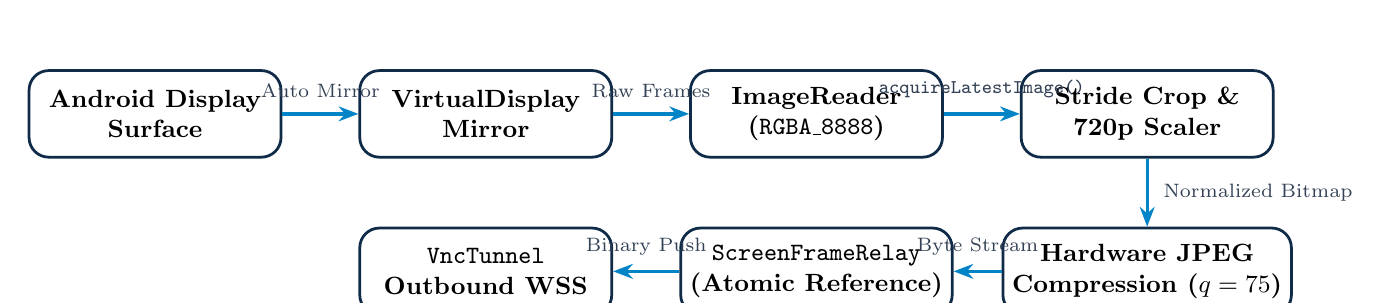
\begin{tikzpicture}[
    stepbox/.style={draw=navyPrimary, fill=white, rounded corners=2.5mm, minimum width=3.2cm, minimum height=1.1cm, align=center, font=\small\bfseries, line width=1pt},
    conn/.style={-{Stealth[length=2.5mm]}, line width=1.2pt, color=tealAccent}
]

\node[stepbox] (surface) at (0,0) {Android Display\\Surface};
\node[stepbox] (virtual) at (4.2,0) {VirtualDisplay\\Mirror};
\node[stepbox] (reader) at (8.4,0) {ImageReader\\(\texttt{RGBA\_8888})};
\node[stepbox] (downsample) at (12.6,0) {Stride Crop \&\\720p Scaler};

\node[stepbox] (compress) at (12.6,-2.0) {Hardware JPEG\\Compression ($q=75$)};
\node[stepbox] (relay) at (8.4,-2.0) {\texttt{ScreenFrameRelay}\\(Atomic Reference)};
\node[stepbox] (ws) at (4.2,-2.0) {\texttt{VncTunnel}\\Outbound WSS};

\draw[conn] (surface) -- node[above=2pt, font=\scriptsize, text=darkSlate] {Auto Mirror} (virtual);
\draw[conn] (virtual) -- node[above=2pt, font=\scriptsize, text=darkSlate] {Raw Frames} (reader);
\draw[conn] (reader) -- node[above=2pt, font=\scriptsize, text=darkSlate] {\texttt{acquireLatestImage()}} (downsample);
\draw[conn] (downsample) -- node[right=2pt, font=\scriptsize, text=darkSlate] {Normalized Bitmap} (compress);
\draw[conn] (compress) -- node[above=2pt, font=\scriptsize, text=darkSlate] {Byte Stream} (relay);
\draw[conn] (relay) -- node[above=2pt, font=\scriptsize, text=darkSlate] {Binary Push} (ws);

\end{tikzpicture}%
}
\caption{Drishti Zero-Root Screen Capture and Frame Relay Pipeline.}
\label{fig:capture}
\end{figure}

\subsubsection{VirtualDisplay Configuration \& Resolution Throttling}
To guarantee fluid frame transmission over bandwidth-constrained cellular links, \texttt{MediaProjectionCaptureService} reads real display dimensions and scales the output surface dynamically:
\begin{lstlisting}[language=Java]
// Cap resolution to 720p maximum width while preserving exact aspect ratio
val scale = minOf(1.0f, MAX_WIDTH.toFloat() / metrics.widthPixels)
screenWidth = (metrics.widthPixels * scale).toInt()
screenHeight = (metrics.heightPixels * scale).toInt()

val reader = ImageReader.newInstance(
    screenWidth, screenHeight,
    PixelFormat.RGBA_8888, 2
)
virtualDisplay = mediaProjection?.createVirtualDisplay(
    "DrishtiCapture", screenWidth, screenHeight, screenDensity,
    DisplayManager.VIRTUAL_DISPLAY_FLAG_AUTO_MIRROR,
    reader.surface, null, handler
)
\end{lstlisting}

\subsubsection{Buffer Stride \& Row Padding Rectification}
Hardware image planes require 64-byte row alignments. Drishti explicitly detects and removes row padding before compression to avoid distorted or skewed frames:
\begin{lstlisting}[language=Java]
val planes = image.planes
val buffer = planes[0].buffer
val pixelStride = planes[0].pixelStride
val rowStride = planes[0].rowStride
val rowPadding = rowStride - pixelStride * screenWidth

val bmp = Bitmap.createBitmap(
    screenWidth + rowPadding / pixelStride, screenHeight,
    Bitmap.Config.ARGB_8888
)
bmp.copyPixelsFromBuffer(buffer)

// Extract pure active screen bounds if padding exists
val cropped = if (rowPadding > 0) {
    Bitmap.createBitmap(bmp, 0, 0, screenWidth, screenHeight).also { bmp.recycle() }
} else {
    bmp
}
\end{lstlisting}

\subsubsection{Decoupled Pub-Sub Transmission with Zero Idle Overhead}
Continuous screen capture on unmanned tablets wastes CPU cycles and generates excessive cellular data traffic. Drishti introduces an in-memory lock-free frame hub (\texttt{ScreenFrameRelay}). When no administrator is actively viewing the device in the dashboard:
\begin{enumerate}
    \item The backend issues a \texttt{viewer\_disconnected} control frame.
    \item \texttt{VncTunnel} unregisters its listener from \texttt{ScreenFrameRelay}.
    \item Frame encoding and transmission immediately cease, reducing idle cellular data consumption to sub-kilobyte heartbeat levels.
\end{enumerate}

\subsection{Pillar 3: Remote Input Injection (AccessibilityService)}
Traditional remote control software injects synthetic touch events by issuing shell commands to \texttt{/dev/input/event*} or executing \texttt{input tap x y} via root. On non-rooted devices, these operations are blocked by SELinux and permission gates.

Drishti utilizes the public Android \textbf{AccessibilityService API} (\texttt{DrishtiAccessibilityService}), which natively supports programmatic gesture dispatching (\texttt{dispatchGesture()}) across the entire OS without root.

\subsubsection{The Android Zero-Length Stroke OEM Defect Workaround}
On multiple OEM Android distributions common in kiosk tablets, an input path consisting solely of \texttt{moveTo(px, py)} is rejected as empty by the system gesture engine. Drishti circumvents this platform bug by programmatically generating a micro-vector delta:
\begin{lstlisting}[language=Java]
fun injectTapPixels(px: Float, py: Float) {
    // Construct a micro-vector path to satisfy Android OEM stroke validators
    val path = Path().apply {
        moveTo(px, py)
        lineTo(px + 0.5f, py + 0.5f)
    }
    val gesture = GestureDescription.Builder()
        .addStroke(GestureDescription.StrokeDescription(path, 0L, 60L))
        .build()
        
    dispatchGesture(gesture, object : GestureResultCallback() {
        override fun onCompleted(gestureDescription: GestureDescription?) {
            Log.i(TAG, "Tap completed at ($px, $py)")
        }
        override fun onCancelled(gestureDescription: GestureDescription?) {
            Log.w(TAG, "Tap cancelled by OS window manager at ($px, $py)")
        }
    }, null)
}
\end{lstlisting}

\subsubsection{Normalized Coordinate Translation}
The web dashboard canvas translates mouse clicks and drag vectors into normalized floating-point coordinates ($nx, ny \in [0.0, 1.0]$). When received by \texttt{VncTunnel}, \texttt{DrishtiAccessibilityService} calculates absolute hardware screen pixels using current \texttt{DisplayMetrics}:
\begin{equation}
px = \mathrm{clamp}\left(nx \times W_{\mathrm{real}},\, 0,\, W_{\mathrm{real}} - 1\right), \quad
py = \mathrm{clamp}\left(ny \times H_{\mathrm{real}},\, 0,\, H_{\mathrm{real}} - 1\right)
\end{equation}
This guarantees pixel-perfect touch alignment across varying tablet aspect ratios and display orientations.

\subsubsection{Global Actions \& Accessible Text Injection}
In addition to touch gestures, the accessibility layer provides system-wide hardware button emulation:
\begin{itemize}[leftmargin=*]
    \item \textbf{Global Navigation:} Direct dispatch of \texttt{GLOBAL\_ACTION\_BACK}, \texttt{GLOBAL\_ACTION\_HOME}, and \texttt{GLOBAL\_ACTION\_RECENTS}.
    \item \textbf{Text Input Dispatch:} The agent locates the active focused input node via \texttt{findFocus(AccessibilityNodeInfo.FOCUS\_INPUT)} and commits the text string directly using \texttt{ACTION\_SET\_TEXT}. If an active accessibility node is unavailable, it automatically stages the string to the Android system clipboard (\texttt{ClipboardManager}).
\end{itemize}

\subsection{Pillar 4: Embedded Local ADB Client (On-Device Wire Protocol)}
While screen sharing and input injection provide comprehensive visual control, technical diagnostics frequently require shell-level access.

\begin{archbox}{How ADB Operates: Local Loopback Architecture}
ADB is not a monolithic binary; it is a networked client/server protocol. The Android system daemon (\texttt{adbd}) listens on local TCP socket port \texttt{5555}. A client communicates using standard wire-protocol packets. 

On a non-rooted device, an app cannot replace \texttt{adbd}, but it can act as an \textbf{ADB Client}. Drishti embeds a pure Kotlin/Java wire-protocol ADB implementation (\texttt{AdbLib}). The agent connects locally via loopback (\texttt{127.0.0.1:5555}), performs standard RSA key exchange, and exposes interactive shell sessions streamed over the outbound WebSocket.
\end{archbox}

\begin{figure}[htbp]
\centering
\resizebox{0.96\textwidth}{!}{%
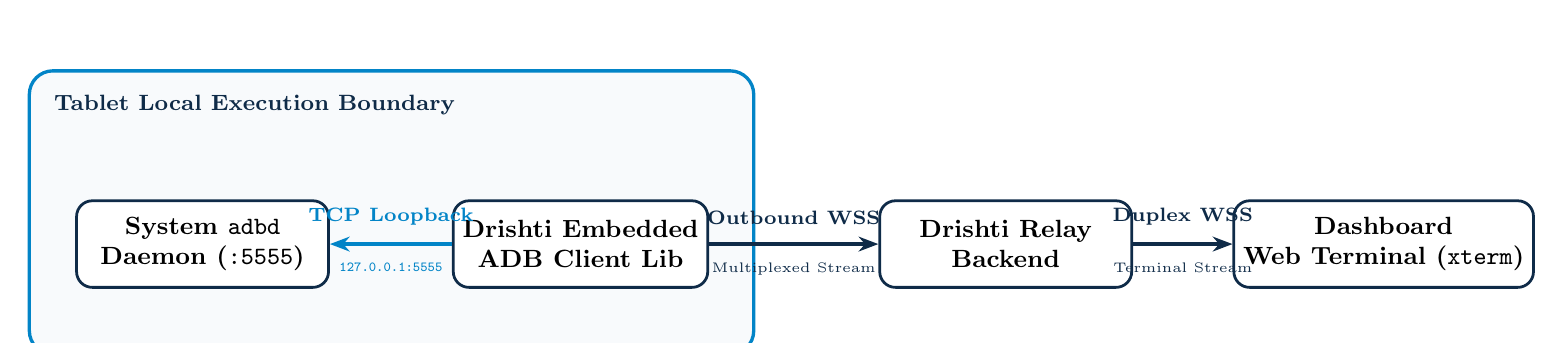
\begin{tikzpicture}[
    agentbox/.style={draw=tealAccent, fill=lightBg, rounded corners=3mm, inner sep=12pt, line width=1.2pt},
    comp/.style={draw=navyPrimary, fill=white, rounded corners=2mm, font=\small\bfseries, align=center, minimum height=1.1cm, minimum width=3.2cm, line width=1pt},
    conn/.style={-{Stealth[length=2.5mm]}, line width=1.2pt}
]

\node[agentbox, minimum width=9.2cm, minimum height=3.6cm] (agentbound) at (0,0) {};
\node[anchor=north west, font=\footnotesize\bfseries, text=navyPrimary] at ([xshift=6pt, yshift=-6pt]agentbound.north west) {Tablet Local Execution Boundary};

\node[comp] (adbd) at (-2.4, -0.4) {System \texttt{adbd}\\Daemon (\texttt{:5555})};
\node[comp] (client) at (2.4, -0.4) {Drishti Embedded\\ADB Client Lib};

\node[comp] (backend) at (7.8, -0.4) {Drishti Relay\\Backend};
\node[comp] (terminal) at (12.6, -0.4) {Dashboard\\Web Terminal (\texttt{xterm})};

\draw[conn, color=tealAccent] (client) -- node[above=3pt, font=\scriptsize\bfseries] {TCP Loopback} 
                                          node[below=3pt, font=\tiny\ttfamily] {127.0.0.1:5555} (adbd);
\draw[conn, color=navyPrimary] (client) -- node[above=3pt, font=\scriptsize\bfseries] {Outbound WSS} 
                                           node[below=3pt, font=\tiny] {Multiplexed Stream} (backend);
\draw[conn, color=navyPrimary] (backend) -- node[above=3pt, font=\scriptsize\bfseries] {Duplex WSS} 
                                            node[below=3pt, font=\tiny] {Terminal Stream} (terminal);

\end{tikzpicture}%
}
\caption{Embedded On-Device ADB Client Loopback Architecture.}
\label{fig:adb}
\end{figure}

\subsection{Pillar 5: Non-Root Application Lifecycle Management}
In \texttt{CommandExecutor.kt}, the agent handles application execution, termination, and updates within non-root constraints:
\begin{itemize}[leftmargin=*]
    \item \textbf{Silent Remote APK Updates:} Because the agent is Device Owner, it can pass downloaded update packages directly to \texttt{android.content.pm.PackageInstaller}. The installation session is committed silently in the background without user interaction.
    \item \textbf{Reliable Kiosk App Launching:} To ensure mission-critical kiosk software remains active, \texttt{CommandExecutor} resolves the target package's launchable intent via \texttt{packageManager.getLaunchIntentForPackage()}. If the OEM launcher component is masked, it leverages the native Android \texttt{monkey} runner (\texttt{monkey -p <pkg> -c android.intent.category.LAUNCHER 1}).
    \item \textbf{Graceful Application Dismissal:} Non-rooted apps cannot execute \texttt{am force-stop} on third-party packages. Drishti resolves this by having \texttt{DrishtiAccessibilityService} inject an immediate \texttt{GLOBAL\_ACTION\_HOME} command, followed by \texttt{ActivityManager.killBackgroundProcesses()}, cleanly dismissing the foreground app without system instability.
\end{itemize}

% =============================================================================
\section{Comprehensive Device Capability Matrix}
% =============================================================================

Table~\ref{tab:comparison} contrasts the operational capabilities, setup requirements, and security profiles across the three device tiers.

\begin{table}[htbp]
\centering
\small
\begin{tabularx}{\textwidth}{p{3.8cm} p{3.4cm} X X}
\toprule
\textbf{Capability / Dimension} & \textbf{Rooted Fleet} & \textbf{Drishti Device Owner (Standard Approach)} & \textbf{Stock Non-Rooted (Unprovisioned Fallback)} \\
\midrule
\textbf{Setup Requirement} & Unlocking bootloader; flashing custom su & One USB command at mounting (10 seconds) & Manual user toggle in system Settings \\
\addlinespace
\textbf{Interactive Screen Share} & Framebuffer / screencap & \textbf{MediaProjection (Silent consent via DPM)} & MediaProjection (Requires physical consent popup) \\
\addlinespace
\textbf{Touch / Gesture Injection} & Direct \texttt{/dev/input} writes & \textbf{AccessibilityService (\texttt{dispatchGesture})} & AccessibilityService (Manual toggle required) \\
\addlinespace
\textbf{Remote Shell Execution} & Full root bash (\texttt{su}) & \textbf{Local ADB loopback client + Sandboxed sh} & Sandboxed sh / temporary Wireless ADB \\
\addlinespace
\textbf{Reboot Survival} & Yes & \textbf{Yes (100\% automated via DPM \& BootReceiver)} & Fragile (OEMs frequently reset developer toggles) \\
\addlinespace
\textbf{Silent APK Installation} & \texttt{pm install} via root & \textbf{PackageInstaller session API via DPM} & Launches system prompt dialog \\
\addlinespace
\textbf{Security Posture} & Severely compromised (SELinux bypassed) & \textbf{Strict Enterprise Grade (SELinux Enforcing)} & Standard Consumer Sandbox \\
\addlinespace
\textbf{Commercial / Banking Feasibility} & Non-compliant (Fails SafetyNet/PCI-DSS) & \textbf{Fully Compliant (Standard Android Enterprise)} & Compliant \\
\bottomrule
\end{tabularx}
\caption{Comparison Matrix: Rooted vs. Drishti Device Owner vs. Unprovisioned Stock.}
\label{tab:comparison}
\end{table}

% =============================================================================
\section{Mounting-Time Provisioning SOP (Standard Operating Procedure)}
% =============================================================================

To operationalize this approach, technicians follow a concise 4-step checklist before mounting tablets into vending machines. The process is fully automated via \texttt{provision\_tablet.sh}.

\begin{figure}[htbp]
\centering
\begin{tcolorbox}[colback=lightBg,colframe=navyPrimary,arc=3mm,title=\textbf{Standard Operating Procedure Checklist (Duration: $\approx 10$ seconds per tablet)}]
\begin{enumerate}[leftmargin=*]
    \item \textbf{Unboxing / Factory State Verification:}
    Ensure the tablet is clean or factory-reset. \textbf{Do not sign into any Google or enterprise accounts.} Connect the tablet to the technician's workstation via USB.
    
    \item \textbf{Enable Developer Debugging:}
    Navigate to \texttt{Settings $\rightarrow$ About Tablet}. Tap \texttt{Build Number} 7 times to reveal Developer Options. Enable \texttt{USB Debugging}.
    
    \item \textbf{Execute Automated Provisioning Script:}
    From the technician's laptop, execute the deployment script:
    \begin{lstlisting}[language=bash]
    bash provision_tablet.sh
    \end{lstlisting}
    The script verifies ADB communication, validates zero enrolled accounts, sideloads the Drishti Agent APK, and assigns Device Owner privileges:
    \begin{lstlisting}[language=bash]
    adb shell dpm set-device-owner com.remoteagent/.AdminReceiver
    \end{lstlisting}
    
    \item \textbf{Mount Tablet into Machine:}
    Disconnect the USB cable. Install the tablet into the vending machine frame. Upon initial network connection, the agent dials the backend relay and registers online automatically.
\end{enumerate}
\end{tcolorbox}
\end{figure}

% =============================================================================
\section{Network Protocol, Streaming \& Scalability}
% =============================================================================

\subsection{Head-of-Line Blocking Prevention via Decoupled Sockets}
Transmitting large binary video frame bursts over the same TCP/WebSocket channel as latency-sensitive control commands causes Head-of-Line (HoL) blocking: an interactive keystroke or tap event can be delayed by hundreds of milliseconds while a heavy 80 KB video frame buffer finishes transmission.

Drishti implements a dual-socket decoupled channel architecture:
\begin{enumerate}
    \item \textbf{Control Channel (JSON text stream):} Dedicated to telemetry, heartbeat, shell I/O, and remote command dispatch. Operates with \texttt{TCP\_NODELAY} enabled to ensure sub-30ms round-trip latency.
    \item \textbf{Screen Frame Channel (Binary stream):} A dedicated WebSocket channel instantiated on demand per active screen-sharing session. Frames are dispatched as raw binary JPEG buffers directly from \texttt{ScreenFrameRelay}.
\end{enumerate}

\subsection{Bandwidth \& Resource Profile}
Table~\ref{tab:bandwidth} details the network throughput and system resource consumption across device operating states.

\begin{table}[htbp]
\centering
\small
\begin{tabularx}{\textwidth}{l X X X}
\toprule
\textbf{Operating State} & \textbf{Network Throughput} & \textbf{CPU Utilization} & \textbf{Memory Footprint} \\
\midrule
\textbf{Standby / Heartbeat Only} & $< 0.5$ KB/sec & $< 0.8\%$ (Idle thread) & $\approx 38$ MB \\
\textbf{Interactive Shell Session} & $1.0 - 5.0$ KB/sec & $1.5 - 3.0\%$ & $\approx 42$ MB \\
\textbf{Active Screen Share (15 FPS, 720p)} & $350 - 650$ KB/sec & $8.0 - 14.0\%$ (GPU/MediaCodec) & $\approx 64$ MB \\
\bottomrule
\end{tabularx}
\caption{Resource and Bandwidth Profiling on Typical Quad-Core ARM Cortex-A55 Tablet.}
\label{tab:bandwidth}
\end{table}

% =============================================================================
\section{Security Architecture \& Cryptographic Boundaries}
% =============================================================================

\subsection{Transport \& Mutual Authentication Security}
\begin{itemize}[leftmargin=*]
    \item \textbf{TLS 1.3 Encryption:} All transport between tablets, backend relays, and administrative dashboards is encrypted via TLS 1.3 with modern cipher suites (AES-256-GCM / ChaCha20-Poly1305).
    \item \textbf{Cryptographic Device Tokens:} Each tablet is provisioned with a unique, high-entropy API key passed via the HTTP header \texttt{x-agent-key} during WebSocket handshakes.
    \item \textbf{Zero Persistent Storage of Visual Frames:} To satisfy privacy standards and prevent data exfiltration, screen frames are never written to disk or recorded on backend relay servers. Frames reside strictly in transient RAM buffers and are immediately overwritten upon transmission.
\end{itemize}

\subsection{Fleet Hardening via Device Owner Governance}
Because the Drishti Agent is enrolled as Device Owner, it can enforce device hardening policies on the vending tablet:
\begin{itemize}[leftmargin=*]
    \item \textbf{Lock Task Mode (Kiosk Pinning):} The agent pins the customer-facing vending application to the foreground, suppressing the system notification shade, navigation bars, and hardware key shortcuts.
    \item \textbf{Uninstall Prevention:} Device Owner status prevents unauthorized users or malware from uninstalling the agent application via standard system settings.
\end{itemize}

% =============================================================================
\section{Conclusion \& Implementation Roadmap}
% =============================================================================

The technical approach detailed in this document provides a robust, enterprise-compliant foundation for remote Android fleet management without device rooting:
\begin{itemize}[leftmargin=*]
    \item \textbf{Root-Free Security:} Eliminates all security, compliance, warranty, and OTA stability liabilities inherent to custom ROMs and \texttt{su} exploits.
    \item \textbf{Deterministic One-Time Setup:} Capitalizes on the standard 10-second mounting-time USB connection to establish permanent Device Owner administrative authority.
    \item \textbf{Full Interactive Control:} Delivers low-latency screen sharing (MediaProjection), unattended touch injection (AccessibilityService), and remote diagnostics (Embedded ADB Client) over outbound-only reverse WebSocket connections.
    \item \textbf{Autonomous Reboot Persistence:} Automatically recovers and resumes operations across unexpected power cycles without human intervention.
\end{itemize}

\vspace{0.3cm}
\begin{tcolorbox}[colback=navyPrimary!5,colframe=navyPrimary,arc=3mm,title=\textbf{Fleet Engineering Roadmap}]
\begin{itemize}[leftmargin=*]
    \item \textbf{Phase 1 (Current Production):} MediaProjection JPEG frame capture, AccessibilityService gesture injection, and Device Owner enrollment via \texttt{provision\_tablet.sh}.
    \item \textbf{Phase 2 (Q3 Enhancement):} Migration of the video pipeline to hardware-accelerated H.264/WebRTC peer-to-peer data channels to reduce backend relay server bandwidth by up to 60\%.
    \item \textbf{Phase 3 (Enterprise Scale):} Integration of zero-touch automated QR enrollment to eliminate USB manual intervention during initial factory unboxing.
\end{itemize}
\end{tcolorbox}

\end{document}
